\documentclass[11pt,a4paper]{article}

\usepackage[T1]{fontenc}
\usepackage[utf8]{inputenc}
\usepackage{lmodern}
\usepackage{microtype}
\usepackage{geometry}
\geometry{top=2.6cm, bottom=2.6cm, left=3cm, right=3cm}

\usepackage{amsmath}
\usepackage{amssymb}
\usepackage{graphicx}
\graphicspath{{Pages/Figures/}}
\usepackage{booktabs}
\usepackage{xcolor}
\usepackage{titlesec}
\usepackage{parskip}
\usepackage{enumitem}
\usepackage{fancyhdr}
\usepackage[numbers,sort&compress]{natbib}
\usepackage[hidelinks]{hyperref}

%% Colours
\definecolor{camblue}{HTML}{003A6C}
\definecolor{rulecol}{HTML}{003A6C}
\definecolor{subtlegray}{HTML}{555555}

%% Section headings with a bold small-caps feel and a thin rule
\titleformat{\section}
  {\normalfont\normalsize\bfseries\color{camblue}}
  {}{0em}
  {}
  [\vspace{1pt}{\color{rulecol}\rule{\linewidth}{0.5pt}}\vspace{-2pt}]
\titlespacing{\section}{0pt}{14pt plus 2pt minus 2pt}{6pt plus 1pt}

%% Footer only
\pagestyle{fancy}
\fancyhf{}
\renewcommand{\headrulewidth}{0pt}
\fancyfoot[R]{\small\color{subtlegray}\thepage}
\fancyfoot[L]{\small\color{subtlegray}Executive Summary}

%% Tighten list spacing
\setlist[itemize]{nosep, leftmargin=1.4em, topsep=4pt}

\begin{document}

%% ---------------------------------------------------------------
%%  HEADER
%% ---------------------------------------------------------------
\thispagestyle{fancy}

\noindent
{\color{rulecol}\rule{\linewidth}{1.8pt}}\\[4pt]
{\LARGE\bfseries Mechanistic Circuits and Concept Geometry\\[2pt]
in an Instruction-Tuned Language Model}\\[6pt]
{\color{rulecol}\rule{\linewidth}{0.5pt}}

\vspace{8pt}
\noindent
{\footnotesize
\textbf{Elisabeta-Iulia (Julia) Dima}\enspace$\cdot$\enspace
MPhil Data Intensive Science\enspace$\cdot$\enspace
University of Cambridge, July 2026
}\\[2pt]
\noindent
{\scriptsize\color{subtlegray}
Supervised by Dr Miles Cranmer and Dr Alessandro Favero\enspace$\cdot$\enspace
DAMTP, Cambridge
}

\vspace{14pt}

%% ---------------------------------------------------------------
\section{Motivation and Scientific Justification}
%% ---------------------------------------------------------------

Large language models can produce correct answers to arithmetic and reasoning
problems without necessarily implementing the intended computation. Output
accuracy therefore cannot distinguish robust internal algorithms from surface
heuristics, memorised templates, or prompt-specific associations. This thesis
studies these aspects in \texttt{Qwen3-4B-Instruct}, an independently trained
instruction-tuned model, using mechanistic interpretability methods that analyse
the residual stream, sparse transcoder features, attribution graphs, activation
patching, and learned input-side interventions.

The work has three purposes. The first is to test whether circuits reported in
Anthropic's \textit{On the Biology of a Large Language Model}~\cite{lindsey2025biology}
transfer to a different instruction-tuned model family. The second is to develop
a general method for locating abstract concepts without relying on a prior
circuit hypothesis. The third is to examine whether learned continuous prefixes
can redirect model behaviour and whether the learned directions are
interpretable relative to the concepts they represent.

%% ---------------------------------------------------------------
\section{Methodology}
%% ---------------------------------------------------------------

The reproducibility study applies the attribution graph framework to Qwen3-4B
through a linearised transcoder model. For two digit addition, sparse features
are scanned across operand grids and token positions to identify range,
residue, lookup, and sum-sensitive activations. Teacher-forced accuracy and
entropy analyses separate errors in the first generated answer token from later
continuation effects. A second reproduction studies multilingual antonym
completion by suppressing and injecting transcoder features corresponding to
operation, operand, and output language.

The concept geometry study introduces a contrastive residual-stream method.
For each concept, matched positive and negative prompt pairs are constructed so
that syntax, length, scale, and answer format are held approximately constant.
The mean residual-stream difference between the two sets defines a layer-wise
concept delta at candidate token anchors. Delta norms are normalised by the
residual activation scale and compared with a permutation null distribution.
Inter-layer cosine similarities then show whether the concept direction remains
stable across depth or rotates. Activation patching tests causal sufficiency by
inserting positive-example residual states into negative examples and measuring
the change in first-token output. Finally, each delta is projected through
transcoder encoder and decoder directions to identify sparse features that read
or write along the concept direction.

This pipeline is applied to three arithmetic contrasts of increasing
representational difficulty, namely carry detection in addition, divisibility by
seven through the greatest common divisor, and residue-class membership modulo
seven. The soft-prompting chapter trains ten learned prefix embeddings with base
model weights frozen, evaluating whether input-side perturbations can correct
residue-class completion, balanced-parentheses judgements, and causal direction
judgements.

%% ---------------------------------------------------------------
\section{Key Findings}
%% ---------------------------------------------------------------

The addition reproduction finds the same high-level digit-pair organisation
reported for Claude 3.5 Haiku. Qwen3-4B reads operand information at digit
positions and recombines decimal residues at the delimiter through lookup-like
and sum-sensitive features. The first answer token is the main source of
difficulty, while later answer tokens become highly confident under teacher
forcing. This supports a lookup-like account of the tested two digit addition
format rather than a sequential carry-propagation account.

The multilingual reproduction shows that semantic operation and operand
components can be edited across English, Chinese, and French. Suppressing
antonym features and injecting synonym features moves completions toward synonym
answers, and changing the operand concept from \textit{small} to \textit{hot} transfers strongly
across languages. In contrast, the attempted output-language edit is weak or
absent. Thus some mechanistic components transfer across languages and model
families, while others depend more strongly on tokenisation, selected layer
range, or prompt surface form.

The concept-localisation results show that concept geometry is not uniform.
For the addition task, stable direction appears around
layers 4 and 5 at the final operand token, survives comparison with the
permutation null baseline, and is causally sufficient under activation patching.
The aligned transcoder features include operand comparison, iso-sum, parity, and
Fourier-like grid structure. GCD divisibility is also localisable, but its
inter-layer cosine matrix shows a block transition, indicating that the
direction rotates rather than persisting as a single axis. At the rotation layer, 
we see divisibility detection patterns, directly correlated with the task. Residue-class
membership does not produce a stable direction above the null band, consistent
with its low first-token accuracy and suggesting that this modular relation is
not encoded as a linearly accessible binary contrast.

\begin{figure}[h]
  \centering
  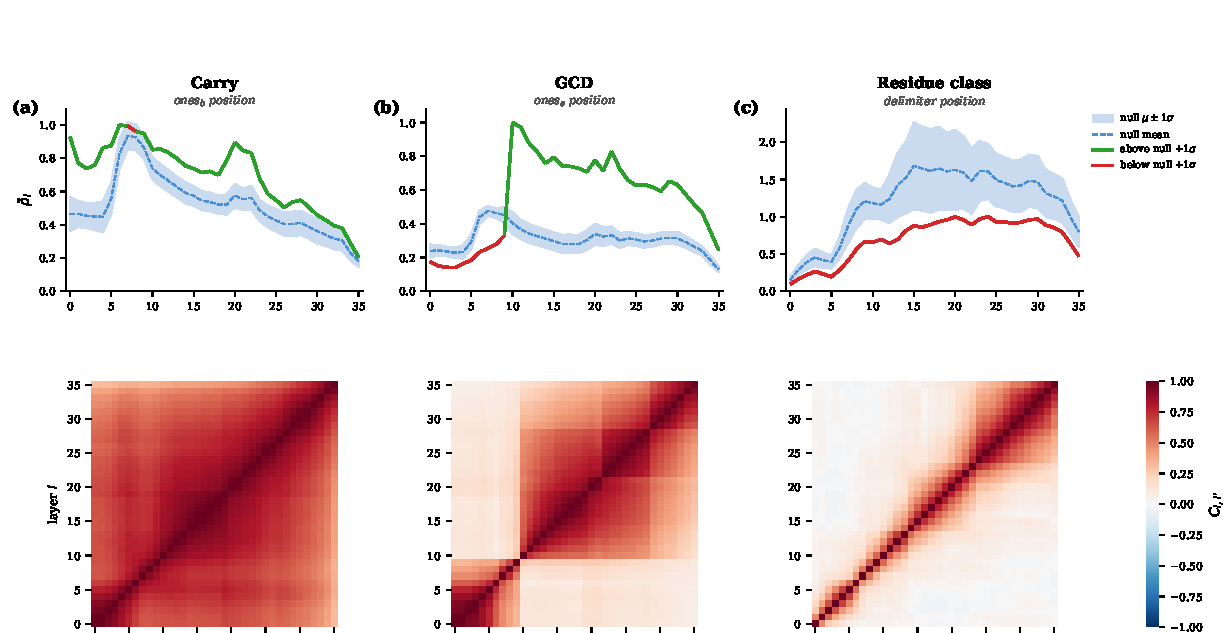
\includegraphics[width=0.86\linewidth]{cosim_patterns_abc.pdf}
  \caption{\small Contrastive residual-stream geometry for carry, GCD
  divisibility, and residue-class membership. Carry shows a stable direction,
  GCD shows a representational rotation, and residue class remains weak relative
  to the null baseline.}
  \label{fig:summary-cosim-patterns}
\end{figure}

The soft-prompting experiments show that learned prefixes can redirect outputs
when the main failure is response format. Accuracy rises from 0\% to 28.6\% on
balanced parentheses and from 0\% to 53.8\% on causal direction judgements.
Residue-class completion changes only from 15.0\% to 16.0\%, while the mean
probability of the correct token decreases. The learned embeddings do not align
with identified concept directions and are not interpretable through transcoder
features, which makes soft prompting effective yet a non-interpretable
transparent knowledge-editing method for our task.

%% ---------------------------------------------------------------
\section{Recommendations and Next Steps}
%% ---------------------------------------------------------------

The main conclusion is that mechanistic structure identified in one model family
can transfer to independently trained instruction-tuned models, but that the
geometry of a target concept strongly conditions whether it can be localised,
patched, or edited. Stable low-rank directions, rotating directions, and absent
linear contrasts require different intervention strategies. This aspect has practical
implications for activation steering, probing, and knowledge editing, where the
existence of an accessible representation should be established before an edit is
attempted.

Future work should test whether the transcoder features identified by delta
projection form causally sufficient circuits when combined with full attribution
graphs. The feature ranking procedure should also account for the
non-orthogonality of decoder vectors and co-activation geometry. Finally, the
contrastive delta method should be applied beyond binary concepts to multi-class and continuous concepts, 
where the geometry may be more complex and the null distribution may need to be
constructed differently.

%% ---------------------------------------------------------------
\section{Research Impact and Conclusion}
%% ---------------------------------------------------------------

Overall, this thesis contributes a reproduction of large-model circuit-tracing
results in Qwen3-4B, a contrastive method for analysing concept geometry across
layers and token positions, and an empirical evaluation of soft prompting as a
residual-stream intervention. Together, these results show that instruction-tuned
models can contain sparse, transferable, and interpretable computational
structure, but also that correct or improved outputs do not imply transparent
internal computation. Mechanistic evaluation must therefore ask where a
representation is encoded, whether it is causally active, and whether an
intervention changes the computation itself or only redirects the surface form of
the answer.

%% ---------------------------------------------------------------
\vspace{8pt}
{\color{rulecol}\rule{\linewidth}{0.5pt}}

\begingroup
\small
\bibliographystyle{unsrt}
\bibliography{thesis}
\endgroup

\end{document}
